
\documentclass[aspectratio=169,10pt,english]{beamer} 
\usetheme{cgs}

\usepackage{babel}
%\usepackage[latin1]{inputenc}
%\usepackage[T1]{fontenc}
\usepackage{graphicx}
\usepackage{amsmath}
\usepackage[labelformat=empty,textfont=small,justification=centering]{caption}
\usepackage[labelformat=empty,textfont=scriptsize,justification=centering]{subcaption}
\usepackage{datetime}
\usepackage{textpos}
\usepackage{tikz}
\usepackage{array}
\usepackage{multirow}
%\usepackage{gitinfo}

\usepackage{inconsolata}
\usepackage{listings}
% code style for glsl

%\RequirePackage[usenames,dvipsnames]{xcolor}

\definecolor{codeKeyword} {rgb}{0.00, 0.00, 1.00} 
\definecolor{codeComment} {rgb}{0.00, 0.50, 0.00} 
\definecolor{codeBkgnd}   {rgb}{0.98, 0.98, 0.98} 
\definecolor{codeFrame}   {rgb}{0.92, 0.92, 0.92} 

\definecolor{codeKeyword1}{rgb}{0.00, 0.00, 0.75}
\definecolor{codeKeyword2}{rgb}{0.50, 0.00, 0.00}
\definecolor{codeKeyword3}{rgb}{0.13, 0.43, 0.52}
\definecolor{codeKeyword4}{rgb}{0.40, 0.40, 0.40}


\definecolor{lightblue}  {rgb}{0.17, 0.57, 0.69}
\definecolor{darkgreen}  {rgb}{0.00, 0.50, 0.00}
\definecolor{lightgrey}  {rgb}{0.66, 0.66, 0.66}

% http://blog.virtualglobebook.com/2011/02/syntax-highlighting-c-and-glsl-source.html

\lstdefinelanguage{glsl}
{
	sensitive=true
,	morekeywords=[1]
{
	attribute, const, uniform, varying,
	layout, centroid, flat, smooth,
	noperspective, break, continue, do,
	for, while, switch, case, default, if,
	else, in, out, inout, float, int, void,
	bool, true, false, invariant, discard,
	return, mat2, mat3, mat4, mat2x2, mat2x3,
	mat2x4, mat3x2, mat3x3, mat3x4, mat4x2,
	mat4x3, mat4x4, vec2, vec3, vec4, ivec2,
	ivec3, ivec4, bvec2, bvec3, bvec4, uint,
	uvec2, uvec3, uvec4, lowp, mediump, highp,
	precision, sampler1D, sampler2D, sampler3D,
	samplerCube, sampler1DShadow,
	sampler2DShadow, samplerCubeShadow,
	sampler1DArray, sampler2DArray,
	sampler1DArrayShadow, sampler2DArrayShadow,
	isampler1D, isampler2D, isampler3D,
	isamplerCube, isampler1DArray,
	isampler2DArray, usampler1D, usampler2D,
	usampler3D, usamplerCube, usampler1DArray,
	usampler2DArray, sampler2DRect,
	sampler2DRectShadow, isampler2DRect,
	usampler2DRect, samplerBuffer,
	isamplerBuffer, usamplerBuffer, sampler2DMS,
	isampler2DMS, usampler2DMS,
	sampler2DMSArray, isampler2DMSArray,
	usampler2DMSArray, struct
}
,	morekeywords=[2]
{
	radians,degrees,sin,cos,tan,asin,acos,atan,
	atan,sinh,cosh,tanh,asinh,acosh,atanh,pow,
	exp,log,exp2,log2,sqrt,inversesqrt,abs,sign,
	floor,trunc,round,roundEven,ceil,fract,mod,modf,
	min,max,clamp,mix,step,smoothstep,isnan,isinf,
	floatBitsToInt,floatBitsToUint,intBitsToFloat,
	uintBitsToFloat,length,distance,dot,cross,
	normalize,faceforward,reflect,refract,
	matrixCompMult,outerProduct,transpose,
	determinant,inverse,lessThan,lessThanEqual,
	greaterThan,greaterThanEqual,equal,notEqual,
	any,all,not,textureSize,texture,textureProj,
	textureLod,textureOffset,texelFetch,
	texelFetchOffset,textureProjOffset,
	textureLodOffset,textureProjLod,
	textureProjLodOffset,textureGrad,
	textureGradOffset,textureProjGrad,
	textureProjGradOffset,texture1D,texture1DProj,
	texture1DProjLod,texture2D,texture2DProj,
	texture2DLod,texture2DProjLod,texture3D,
	texture3DProj,texture3DLod,texture3DProjLod,
	textureCube,textureCubeLod,shadow1D,shadow2D,
	shadow1DProj,shadow2DProj,shadow1DLod,
	shadow2DLod,shadow1DProjLod,shadow2DProjLod,
	dFdx,dFdy,fwidth,noise1,noise2,noise3,noise4,
	EmitVertex,EndPrimitive
}
,	morekeywords=[3]
{
	gl_VertexID,gl_InstanceID,gl_Position,
	gl_PointSize,gl_ClipDistance,gl_PerVertex,
	gl_Layer,gl_ClipVertex,gl_FragCoord,
	gl_FrontFacing,gl_ClipDistance,gl_FragColor,
	gl_FragData,gl_MaxDrawBuffers,gl_FragDepth,
	gl_PointCoord,gl_PrimitiveID,
	gl_MaxVertexAttribs,gl_MaxVertexUniformComponents,
	gl_MaxVaryingFloats,gl_MaxVaryingComponents,
	gl_MaxVertexOutputComponents,
	gl_MaxGeometryInputComponents,
	gl_MaxGeometryOutputComponents,
	gl_MaxFragmentInputComponents,
	gl_MaxVertexTextureImageUnits,
	gl_MaxCombinedTextureImageUnits,
	gl_MaxTextureImageUnits,
	gl_MaxFragmentUniformComponents,
	gl_MaxDrawBuffers,gl_MaxClipDistances,
	gl_MaxGeometryTextureImageUnits,
	gl_MaxGeometryOutputVertices,
	gl_MaxGeometryOutputVertices,
	gl_MaxGeometryTotalOutputComponents,
	gl_MaxGeometryUniformComponents,
	gl_MaxGeometryVaryingComponents,gl_DepthRange
}
,	morecomment=[l]{//}
,	morecomment=[s]{/*}{*/}
,	morecomment=[l][keywordstyle4]{\#}
,	morecomment=[s][keywordstyle4]{\"}{\"}
}

\lstset{
	basicstyle       = \scriptsize\ttfamily
,	backgroundcolor  = \color{codeBkgnd}
,	rulecolor        = \color{codeFrame}
,	keywordstyle     = \color{codeKeyword}
,	commentstyle     = \color{codeComment}
,	keywordstyle		 = [1]\color{codeKeyword1}
,	keywordstyle		 = [2]\color{codeKeyword2}
,	keywordstyle		 = [3]\color{codeKeyword3}
,	keywordstyle		 = [4]\color{codeKeyword4}
,	numberbychapter  = true
,	numbersep        = 8pt
,	tabsize          =  4          
,	numbers          = left
,	numberstyle      = \tiny
,	frame            = single
,	framesep         =  4pt
, xleftmargin=\parindent
,	xleftmargin      = 16pt
, framexleftmargin = 16pt
,	abovecaptionskip = \medskipamount
, firstnumber      = 1
, stepnumber       = 1
}


\hypersetup{bookmarksopen=false}

\providecommand*{\what}[1]{\widehat{#1}}
\providecommand*{\wtilde}[1]{\widetilde{#1}}

\title{Grafikprogrammierung mit C++ und OpenGL}
\author{Stefan Buschmann, Daniel Limberger, Amir Semmo}
\institute{Hasso-Plattner-Institut}
\date{SoSe~2013}

\setbeamercolor{postit}{fg=black,bg=white}

\newcommand<>{\fullsizegraphic}[2]
{
	\begin{tikzpicture}[remember picture,overlay]
	\node[at=(current page.center)]
	{
		\includegraphics[width=\paperwidth]{#1}
	};
	\end{tikzpicture}

	\vspace{-0.33\paperheight}\hfill
	\begin{beamercolorbox}[wd=0.5\paperwidth,ht=11mm,dp=1ex,right,rightskip=1cm]{postit}
		\fontsize{8mm}{0}\selectfont  \uppercase{\textbf{#2}}
		\vspace{2mm}
	\end{beamercolorbox}
	\hspace{-2cm}
}

\newcommand<>{\grayout}{\textcolor{gray}}

\subtitle{Seminar Introduction: Lectures, Hands-On, Collaborative Open Source Project}
\titlegraphic{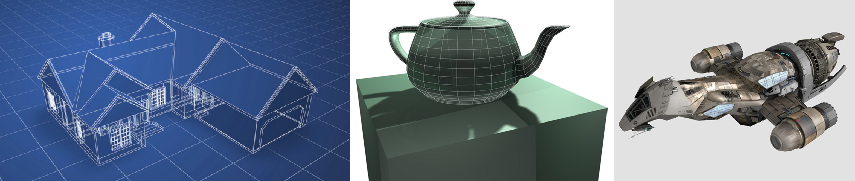
\includegraphics[width=\linewidth]{intro/intro_teaser}}

\begin{document}

\begin{frame}[plain]
	\titlepage
\end{frame}


\begin{frame}{Agenda}
	
	\begin{figure}
	
		\centering
		\begin{subfigure}[b]{0.3\textwidth}
			\centering
			
\includegraphics[width=\textwidth]{intro/concept}
			\caption{\normalsize 1) Seminar Concept}
		\end{subfigure}%
		\quad
		\begin{subfigure}[b]{0.3\textwidth}
			\centering
			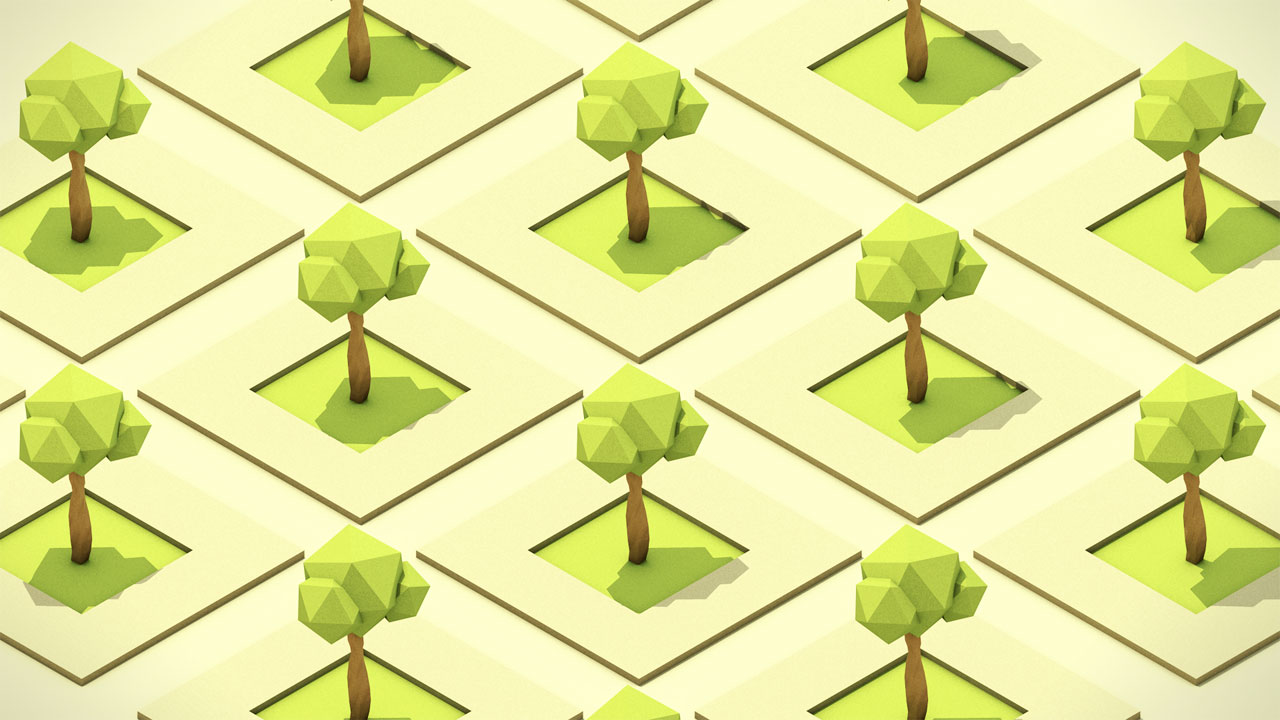
\includegraphics[width=\textwidth]{intro/survey}
			\caption{\normalsize 2) Skill Survey}
		\end{subfigure}
		\quad
		\begin{subfigure}[b]{0.3\textwidth}
			\centering
			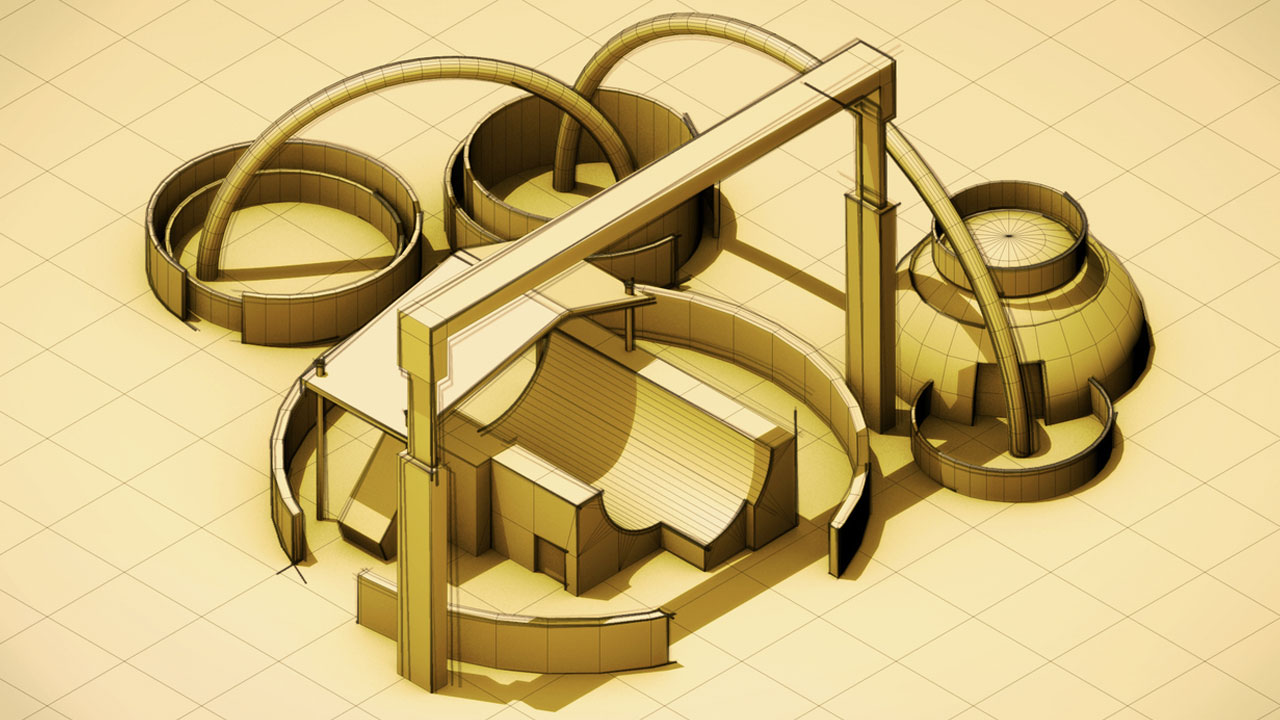
\includegraphics[width=\textwidth]{intro/structure}
			\caption{\normalsize 3) Seminar Structure}
		\end{subfigure}

	\end{figure}

	\begin{figure}
	
		\centering
		\begin{subfigure}[b]{0.3\textwidth}
			\centering
			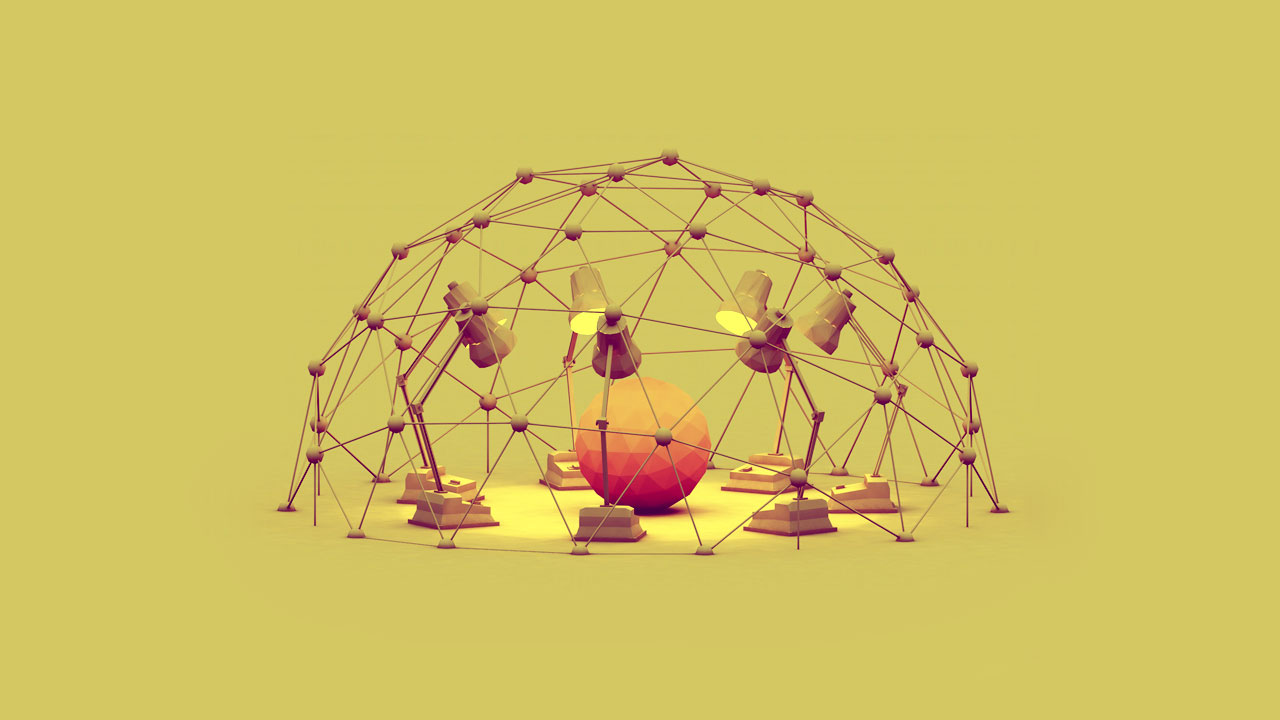
\includegraphics[width=\textwidth]{intro/project}
			\caption{\normalsize 4) Collaborative Project}
		\end{subfigure}%
		\quad
		\begin{subfigure}[b]{0.3\textwidth}
			\centering
			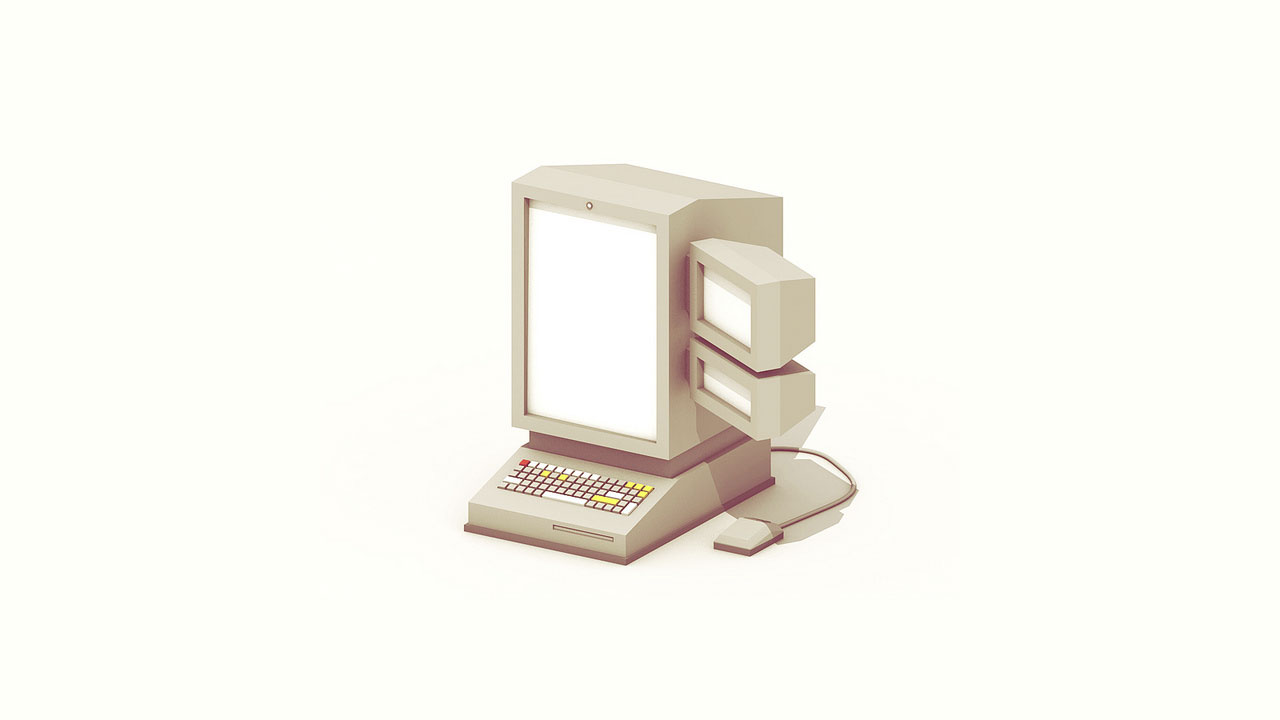
\includegraphics[width=\textwidth]{intro/about}
			\caption{\normalsize 5) Your Participation}
		\end{subfigure}
		\quad
		\begin{subfigure}[b]{0.3\textwidth}
			\centering
			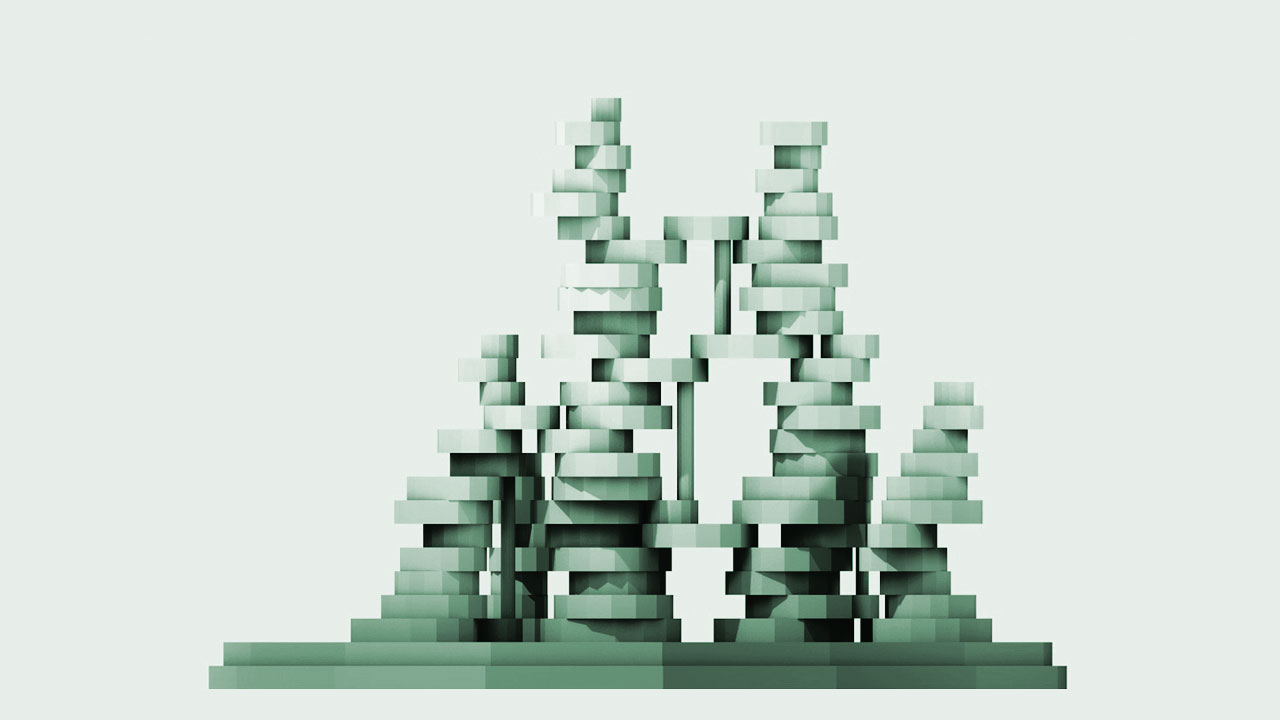
\includegraphics[width=\textwidth]{intro/ideas}
			\caption{\normalsize 6) Getting Started}
		\end{subfigure}

	\end{figure}
	
\end{frame}


% -------- -------- -------- -------- -------- -------- -------- --------

\begin{frame}[plain]
	\fullsizegraphic{intro/concept}{Concept}
\end{frame}


\begin{frame}{Seminar Concept}
	
	\center
	\begin{columns}
		\begin{column}{0.3\textwidth}

			\visible<6>{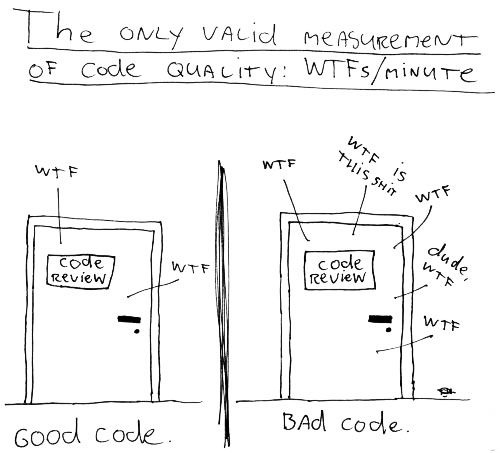
\includegraphics[width=\textwidth]{intro/wtfperminute}}

		\end{column}
		\begin{column}{0.6\textwidth}

			You are going to
			\bigskip

			\pause
			\small
			\begin{itemize}

				\item get advanced C/C++ ($2/3$) and OpenGL ($1/3$) input.\smallskip
				\pause
				\item work on a collaborative, open source CG project.\smallskip
				\pause
				\item develop cross plattform (GCC, MSVC, XCode, etc.).\smallskip
				\pause
				\item know how to handle Qt and CMake.\smallskip
				\pause
				\item assess, justify, discuss, and criticize source code.\smallskip

			\end{itemize}

		\end{column}
	\end{columns}	

\end{frame}


\begin{frame}{Hello World}
	
	\center\Large
	This seminar is all \textbf{NEW} - new content, new slides, new project - and You will (if so) participate in its \textbf{first pass}.
	\vspace{1cm}
	
	\pause\small
	\textbf{Your interests, ideas, and feedback} are valueable for seminar quality and success.
	
\end{frame}


% -------- -------- -------- -------- -------- -------- -------- --------

\begin{frame}[plain]
	\fullsizegraphic{intro/survey}{Skill Survey}
\end{frame}


% Survey Should be based on Yes/No Questions

\begin{frame}[fragile]{Skill Survey 1/4 - C/C++ Experience}
	
	\pause
	WHO has worked on more than two C/C++ \textbf{projects}?\bigskip

	\pause
	WHO knows the meaning of more than half of the following C/C++ \textbf{keywords}?
	\begin{lstlisting}[language=C++]
		auto break class const constexpr const_cast continue delete default 
		dynamic_cast enum explicit friend inline mutable namespace nullptr 
		operator overwrite private protected reinterpret_cast signed sizeof 
		static static_cast template typedef typename union using virtual void
	\end{lstlisting}\bigskip

	\pause
	WHO is familiar with more than half of the following \textbf{concepts}?
	
	\begin{scriptsize}
		Unnamed Namespaces; References; Operator Overloading; Function Pointer; Multiple Inheritance;
		Pure Virtual; Smart-Pointer; Memory Fragmentation; Run Time Type Information; Forward Declarations;
		Precompiled Headers; Macros; Include Guards; Containers and Iterators; Lazy Initialization;
	\end{scriptsize}\bigskip

	\pause
	WHO has worked on at least one \textbf{platform independent} C/C++ project?\bigskip

	\pause
	WHO has worked with \textbf{CMake}?

\end{frame}


\begin{frame}[fragile]{Skill Survey 2/4 - C/C++ Tests}

	\pause
	\begin{lstlisting}[language=C++]
		int a = 13, b = 013;
		a ^= b ^= a ^= b;
	\end{lstlisting}

	\pause
	\begin{lstlisting}[language=C++]
		const QString t("Hello World");
		const char * c(t.toLocal8Bit().constData());
	\end{lstlisting}

	\pause
	\begin{lstlisting}[language=C++]
		const float  f(const float  x) { 
		  return 3.f * x; } 
		const double f(const double x) { 
		  return 2.  * x; }

		f(2); // ? 
	\end{lstlisting}

	\pause
	\begin{lstlisting}[language=C++]
		void foo(int const * a, int * const b);
	\end{lstlisting}

\end{frame}


\begin{frame}[fragile]{Skill Survey 3/4 - Graphics Experience}
	
	\pause
	WHO has worked on more than two \textbf{projects} with graphics programming involved?\bigskip

	\pause
	WHO knows which of the following functions are \textbf{not deprecated} in OpenGL 3.2?
	\begin{lstlisting}[language=C++]
		Rotate Begin End GenLists Vertex MultiTexCoord LoadIdentity PushMatrix InterleavedArrays
		MultTransposeMatrix Rotate Scale Translate TexGen Material Light ColorMaterial ShadeModel
	\end{lstlisting}\medskip

	\pause
	WHO has used the GPU for \textbf{computation}al stuff?\bigskip

	\pause
	WHO is familiar with more than half of the following rendering \textbf{concepts}?\par
	\begin{scriptsize}
		Fragment; Texel; Pixel; Image; Texture; Path Tracing; Immutable Texture; Vertex Buffer Object; Ray Casting;
		Transform Feedback; Instancing; Shader; Program; Pipeline; Atomic Counter; Texture Views; Bindless Texture; 
	\end{scriptsize}\bigskip

	\pause
	WHO has seen at least one of these \textbf{guys}?\medskip 

	% pause does not work for graphics
	\visible<6>{
\includegraphics[width=0.4\textwidth]{intro/opengl}}

\end{frame}


\begin{frame}[fragile]{Skill Survey 4/4 - Graphics Tests}

	\pause
	% what do they do - deprecation? warnings?
	% b is deprecated
	% d needs to be initialized - warning
	\begin{lstlisting}[language=glsl]
		     in vec3 a;
		varying vec3 b;
		uniform vec3 c;
		  const vec3 d;
		    out vec3 e;
	\end{lstlisting}

	\pause
	% what does it? does this work? warning? deprecation?
	% mixes colores with a * 0.8 + d * 0.2
	% does not work, since mix returns vec3 and fragcolor is vec4
	% is deprecated, since gl_FragColor is not used anymore -> specify out
	\begin{lstlisting}[language=glsl]
		gl_FragColor = mix(a, d, 0.2);
	\end{lstlisting}

	\pause
	% what's the difference?
	% none -> a is defaulted to location 0
	\begin{lstlisting}[language=glsl]
		                     out vec4 a;
		layout(location = 0) out vec4 b;
	\end{lstlisting}

	\pause
	% what is the behaviour?
	% Swizzle operators
	% Noise not implemented
	% HARDWARE-BASED CONDITIONAL BRANCHING
	\begin{lstlisting}[language=glsl]
		vec2 n = noise2(fragID);
		vec4 t;
		
		if(n < 0.333)
		  t = texelFetch(sampler, n.yx);
		else
		  t = texelFetch(sampler, n.xy);
	\end{lstlisting}

\end{frame}


% -------- -------- -------- -------- -------- -------- -------- --------

\begin{frame}[plain]
	\fullsizegraphic{intro/structure}{Structure}
\end{frame}


\begin{frame}[fragile]{Seminar Structure}

	\begin{columns}
		\begin{column}{0.5\textwidth}

			\begin{figure}
				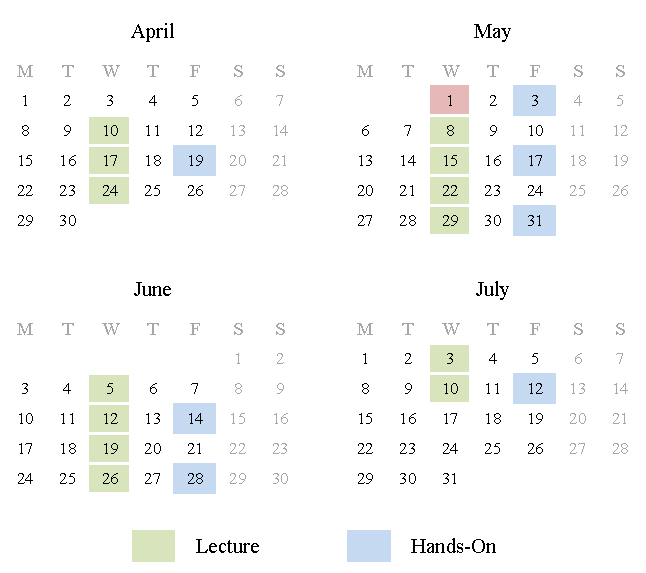
\includegraphics[width=\textwidth]{intro/calendar}
			\end{figure}

		\end{column}
		\begin{column}{0.5\textwidth}

			\small
			\begin{itemize}
			
				\pause
				\item \textbf{13 $\times$ Lecture}\\
					C++, CMake, OpenGL/GLSL, Qt,\\
					code riddles and assessments
					\smallskip

				\pause
				\item \textbf{Individual Tasks} (2 - 3 $\times$ each)\\
					Contribution to a collaborative\\
					open source project: \emph{CGSee}
					\smallskip

				\pause
				\item  \textbf{7 $\times$ Hands-On}\\
					Programming sessions with everyone:\\
					working on individual task, joint inspection of and feedback for ideas and results.
					\smallskip
				
				\pause
				\item \textbf{Short Talks} (3 + 2 min)\\
					Consecutive short presentations\\
					of \emph{CGSee} contributions.\\ % each lecture beginning with one or two 5 minute talks.

			\end{itemize}

		\end{column}
	\end{columns}

\end{frame}


\begin{frame}{Seminar Content}
	
	\small
	
	\begin{columns}
		\begin{column}{0.5\textwidth}
	
			\begin{table}
				\centering
					\begin{tabular}{p{0.1\textwidth}p{0.8\textwidth}}

					04/10 & Introduction, project and process, issues for \textbf{individual tasks}\smallskip\\
					04/17 & Initial \textbf{tasks assignment}, source introduction, and project planning\smallskip\\
					04/19 & Review \& hands-on\smallskip\\

					\hline\smallskip\\

					04/24 & C++\_1\smallskip\\
					\grayout{05/01} & \grayout{\texttt{nullptr}}\smallskip\\
					05/03 & \grayout{Review \& hands-on}\smallskip\\
					05/08 & OpenGL\_1\smallskip\\
					05/15 & C++\_2\smallskip\\
					05/17 & \grayout{Review \& hands-on}\smallskip\\
					05/22 & Cross-Platform\smallskip\\

					\end{tabular}
			\end{table}
		
		\end{column}
		\begin{column}{0.5\textwidth}

			\begin{table}
				\centering
					\begin{tabular}{p{0.1\textwidth}p{0.8\textwidth}}

					05/29 & Qt\_1\smallskip\\
					05/31 & \grayout{Review \& hands-On}\smallskip\\
					06/05 & OpenGL\_2\smallskip\\
					06/12 & CPP\_3\smallskip\\
					06/14 & \grayout{Review \& hands-On}\smallskip\\
					06/19 & OpenGL\_3\smallskip\\
					06/26 & C++\_4\smallskip\\
					06/28 & \grayout{Review \& hands-On}\smallskip\\
					07/03 & C++\_5\smallskip\\

					\hline\smallskip\\

					07/10 & \textbf{Buffer zone, discussion, feedback}\smallskip\\
					07/12 & \textbf{CGSee evaluation, status review, future work, feedback}\smallskip\\

				\end{tabular}
			\end{table}

		\end{column}
	\end{columns}
		
\end{frame}


\begin{frame}{Content References (Books)}

	\center
	
	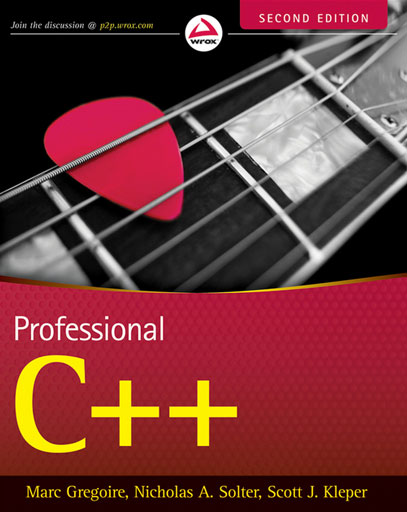
\includegraphics[width=0.15\textwidth]{books/profcpp}
	~
	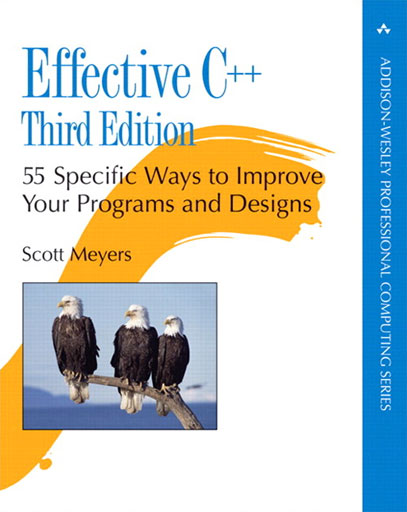
\includegraphics[width=0.15\textwidth]{books/effective}
	~
	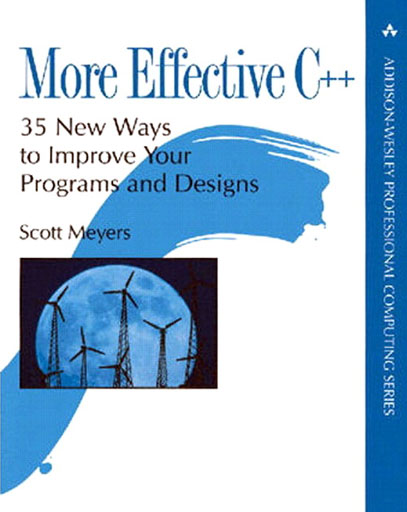
\includegraphics[width=0.15\textwidth]{books/moreeffective}
	~
	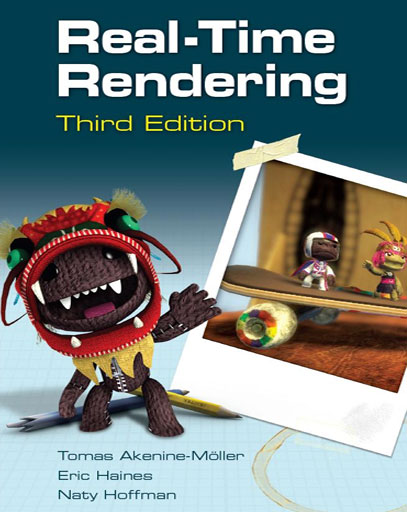
\includegraphics[width=0.15\textwidth]{books/realtime}
	~
	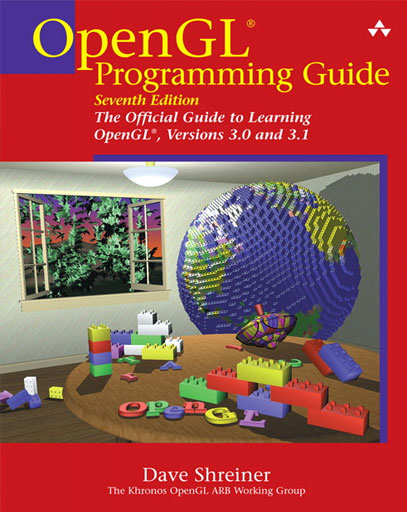
\includegraphics[width=0.15\textwidth]{books/red}
	~
	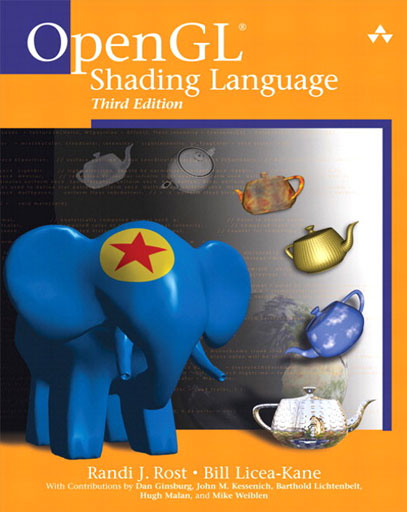
\includegraphics[width=0.15\textwidth]{books/orange}
	
	\medskip

	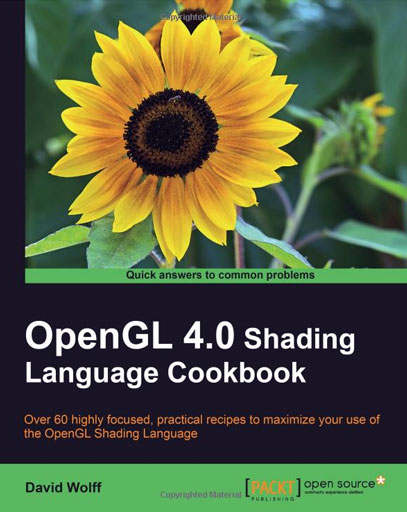
\includegraphics[width=0.15\textwidth]{books/oglshadingcook}	
	~
	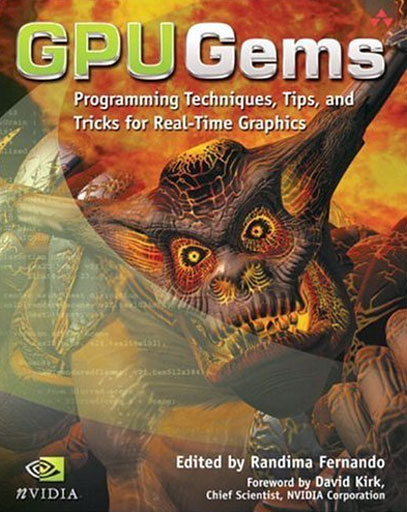
\includegraphics[width=0.15\textwidth]{books/gems1}	
	~
	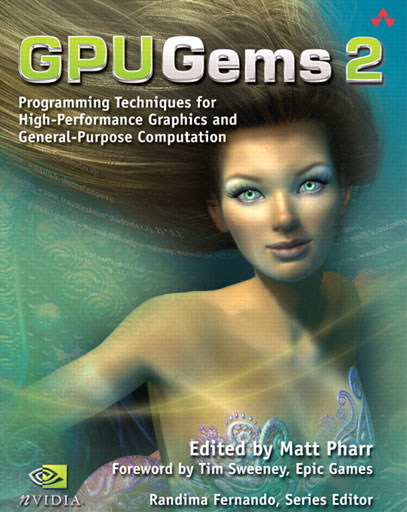
\includegraphics[width=0.15\textwidth]{books/gems2}	
	~
	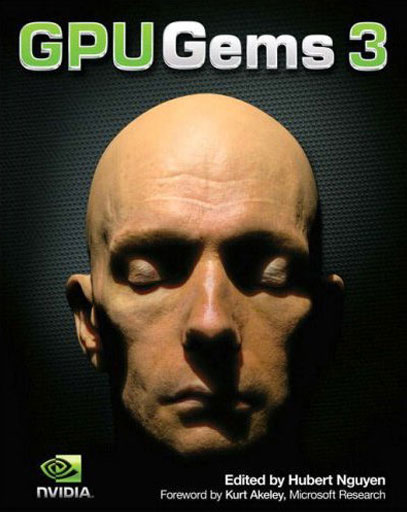
\includegraphics[width=0.15\textwidth]{books/gems3}	
	~
	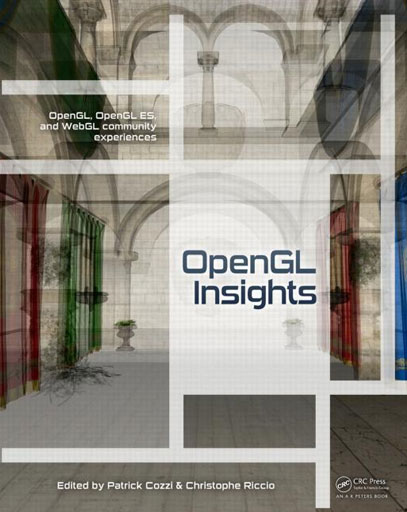
\includegraphics[width=0.15\textwidth]{books/oglinsights}	
	~
	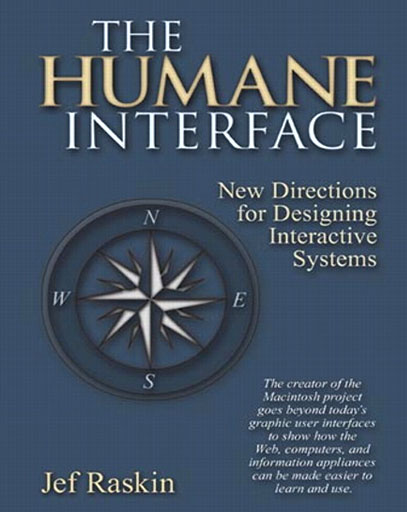
\includegraphics[width=0.15\textwidth]{books/humaninterface}
	
\end{frame}


\begin{frame}{About the Teachers}

	% More personal? - Books/Games/Movies
	\begin{figure}
	
		\centering
		\begin{subfigure}[b]{0.3\textwidth}
			\centering
			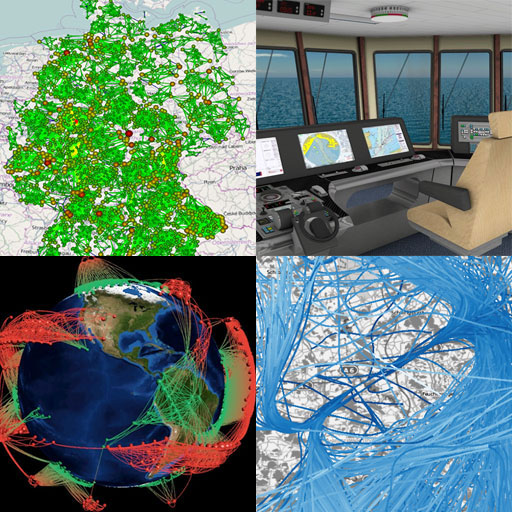
\includegraphics[width=\textwidth]{intro/stefan}
			\caption{\normalsize \textbf{Stefan Buschmann}}
			%\\\bigskip\tiny Hyperion Series, 1984, Liebesfluchten\\BF3, S.t.a.l.k.e.r., Journey, ME\\Breaking Bad, Firefly, Coupling\\Soundtracks, Electro Stuff, Pop\\Drive, Killing Them Softly, Shame}
		\end{subfigure}%
		\quad
		\begin{subfigure}[b]{0.3\textwidth}
			\centering
			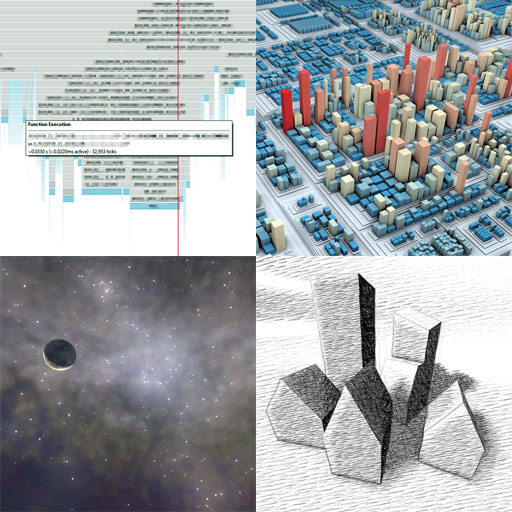
\includegraphics[width=\textwidth]{intro/daniel}
			\caption{\normalsize \textbf{Daniel Limberger}}
			%\\\bigskip\tiny Hyperion Series, 1984, Liebesfluchten\\BF3, S.t.a.l.k.e.r., Journey, ME\\Breaking Bad, Firefly, Coupling\\Soundtracks, Electro Stuff, Pop\\Drive, Killing Them Softly, Shame}
		\end{subfigure}
		\quad
		\begin{subfigure}[b]{0.3\textwidth}
			\centering
			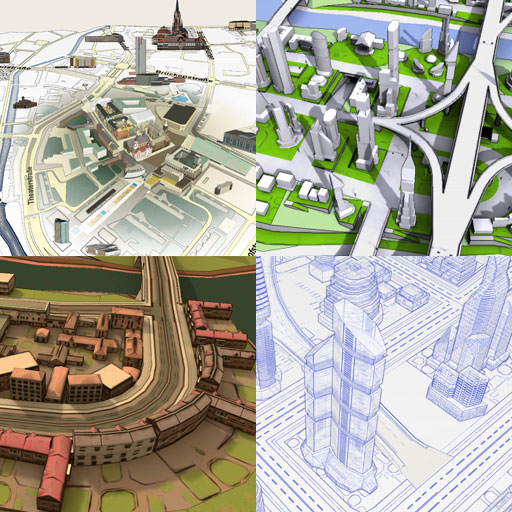
\includegraphics[width=\textwidth]{intro/amir}
			\caption{\normalsize \textbf{Amir Semmo}}
			%\\\bigskip\tiny Hyperion Series, 1984, Liebesfluchten\\BF3, S.t.a.l.k.e.r., Journey, ME\\Breaking Bad, Firefly, Coupling\\Soundtracks, Electro Stuff, Pop\\Drive, Killing Them Softly, Shame}
		\end{subfigure}

	\end{figure}

\end{frame}


% -------- -------- -------- -------- -------- -------- -------- --------

\begin{frame}[plain]
	\fullsizegraphic{intro/project}{Project}
\end{frame}


\begin{frame}{Collaborative Open Source Project}
	
	\center
	
	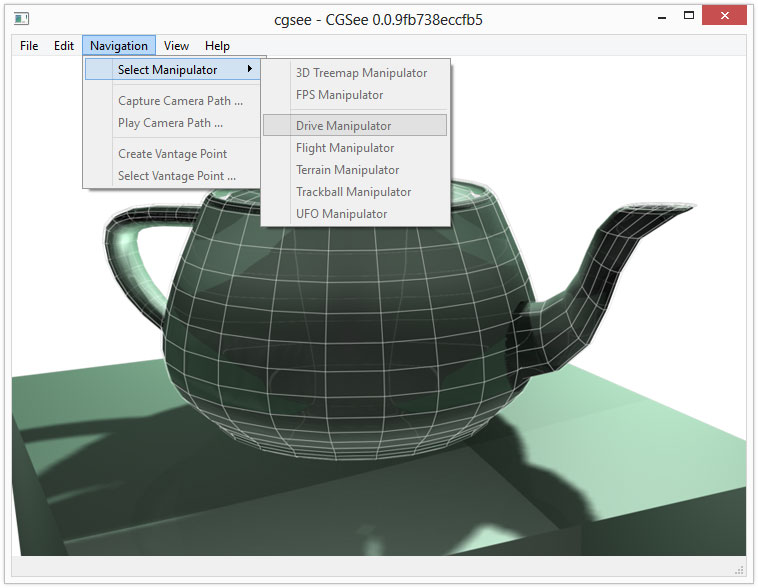
\includegraphics[width=0.3\textwidth]{intro/mock_00}

	\Huge \textbf{CGSee}\\
	\smallskip
	\small Working Title
	\bigskip
	
	\Large
	Free open source viewer for computer graphics related data,\\intended to become a Deep Exploration replacement.

\end{frame}


\begin{frame}{Project Motivation}
	
	\begin{itemize}
		\item Rendering, navigation, and conversion of 3D geometry
		\bigskip
		\pause
		\item 3D Geometry is exchanged and used in various areas of CG.\\Movies, games, logos, CAD, evaluation of rendering techniques
		\bigskip
		\pause
		\item 3D file format hell % e.g. coordinate systems, mostly only partial support
		\item 3D meshes vs. 3D scenes % materials, animation, graph based vs groups and lists, free-form
		\item image based and procedural matarials
		\item animation and dynamics
	\end{itemize}

\end{frame}


\begin{frame}{Project Motivation}

	\center
	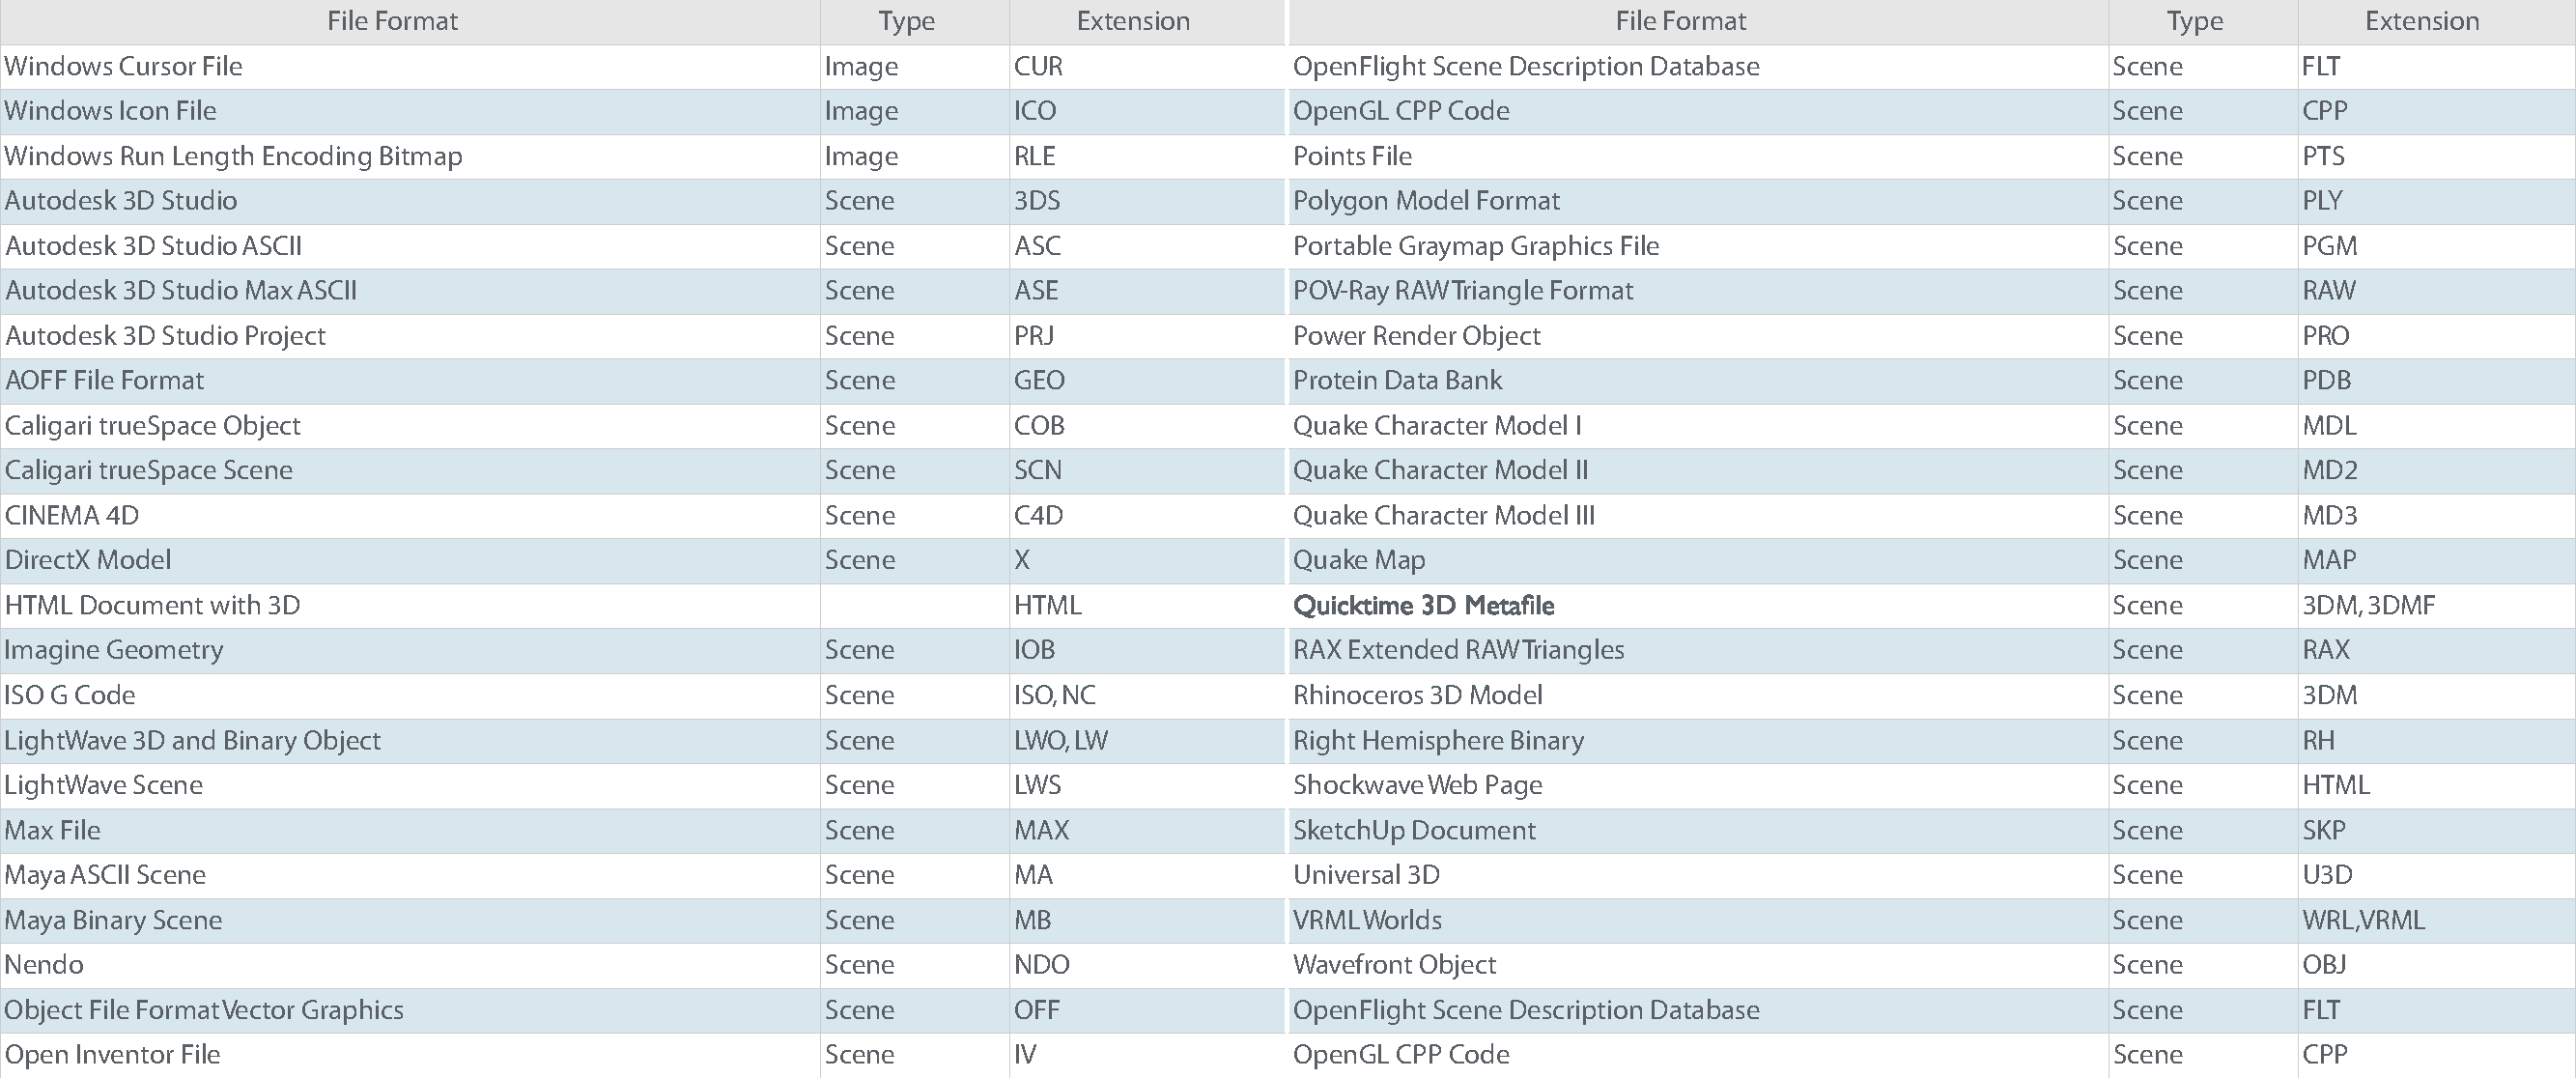
\includegraphics[width=\textwidth]{intro/fileformats}

\end{frame}


\begin{frame}{Deep Exploration - RIP}
	
	\center
	
	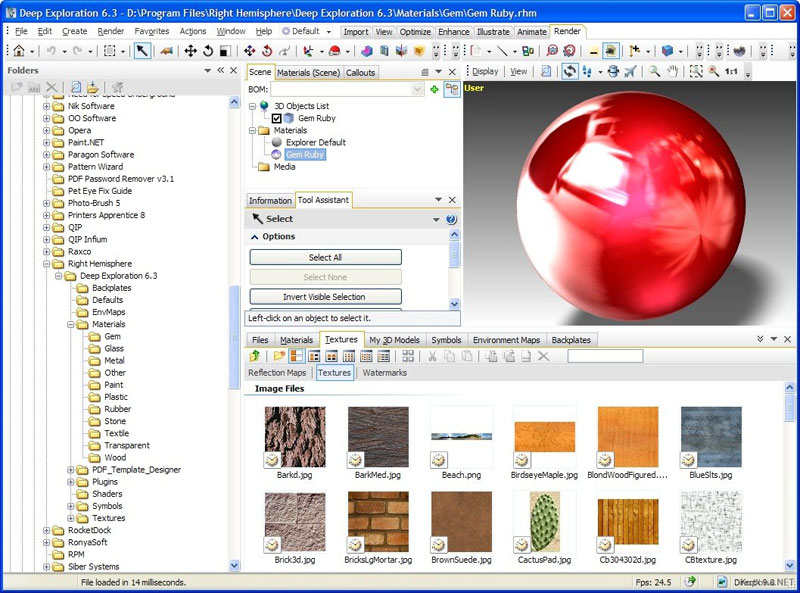
\includegraphics[width=0.45\textwidth]{intro/deepexp_01}
	\quad
	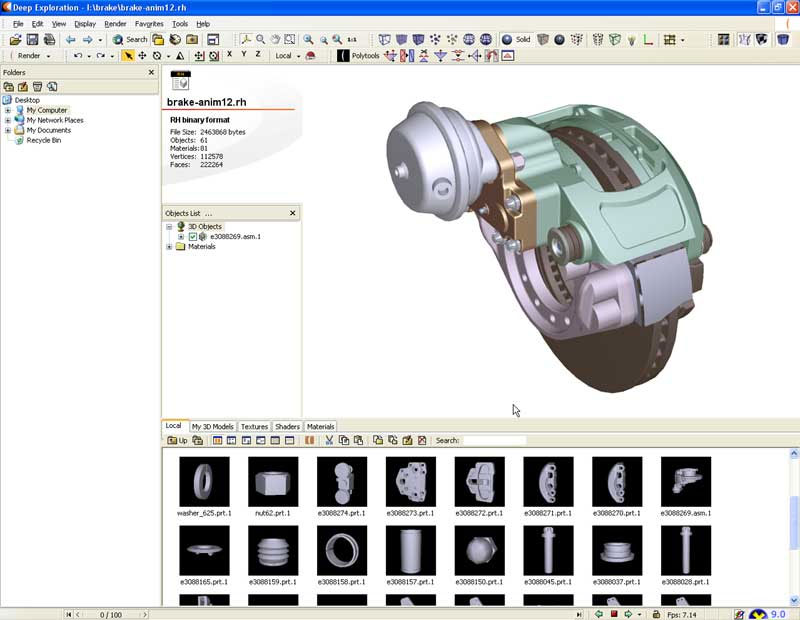
\includegraphics[width=0.45\textwidth]{intro/deepexp_02}
	\bigskip
	
	Right Hemisphere got aquired by SAP in 2011.\\\scriptsize\medskip
	(Their products are now used for SAP Visual Enterprise)

\end{frame}


\begin{frame}{Project Alternatives}
	
	\Large
	Alternatives: 3D-Tool; Quick3D; Solid; Solid Works; Solid Edge Viewer; Rotor 3D Viewer; ...; 
	\bigskip

	\normalsize
	There are currently no similarly good alternatives: Either only CAD oriented, not free, few formats, bad export, bad navigation, old code base, bad UI, etc., ...

\end{frame}


\begin{frame}{Collaborative Open Source Project}

	\begin{columns}
		\begin{column}{0.5\textwidth}

			Requirements for \textbf{CGSee}:
			\bigskip

			\begin{itemize}
				\item clean and minimal ui
				\item common formats for import and export
				\item basic manipulation capabilites\\(e.g., mirroring, geometry fixes, etc.)
				\item efficient and beautiful rendering
				\item exploration tools\\(e.g., filtering, navigation, scene structure)
				\item measurements
				\item ...
			\end{itemize}	
			
		\end{column}
		\begin{column}{0.5\textwidth}

			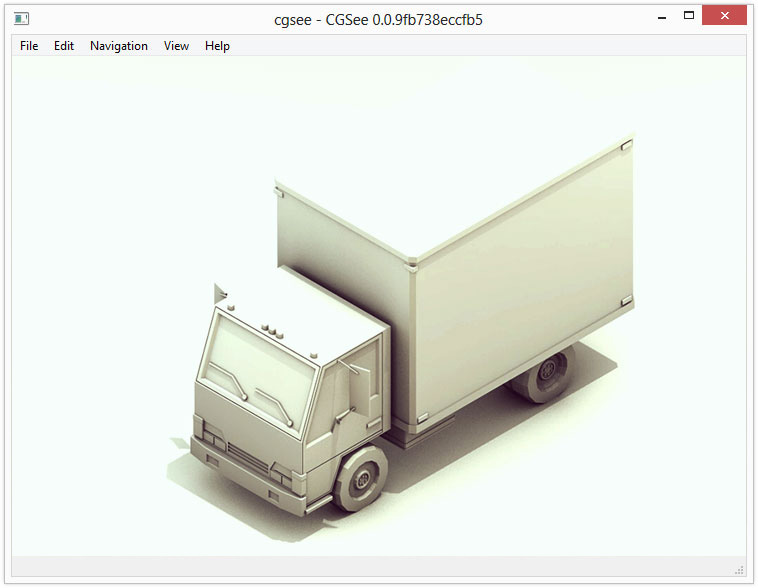
\includegraphics[width=\textwidth]{intro/mock_06}
			
		\end{column}
	\end{columns}

\end{frame}


\begin{frame}{Inspiration}

	\center

	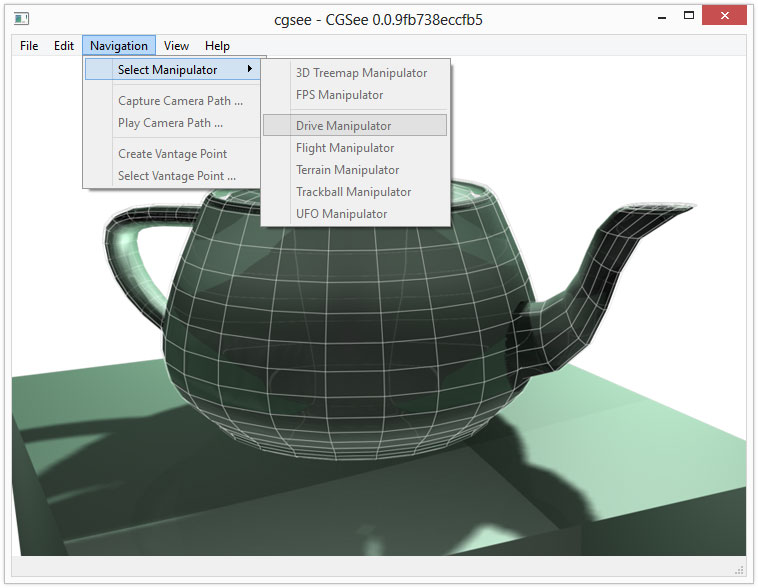
\includegraphics[width=0.3\textwidth]{intro/mock_00}
	~
	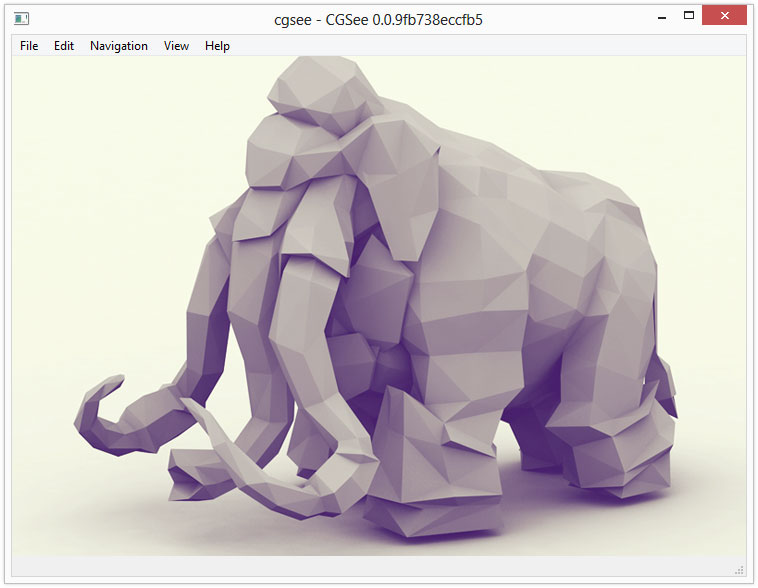
\includegraphics[width=0.3\textwidth]{intro/mock_01}
	~
	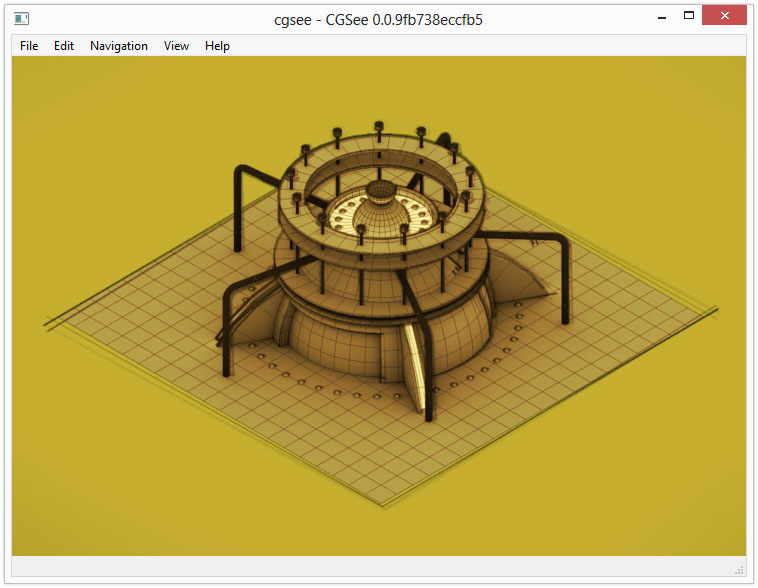
\includegraphics[width=0.3\textwidth]{intro/mock_02}
		
	\medskip
	
	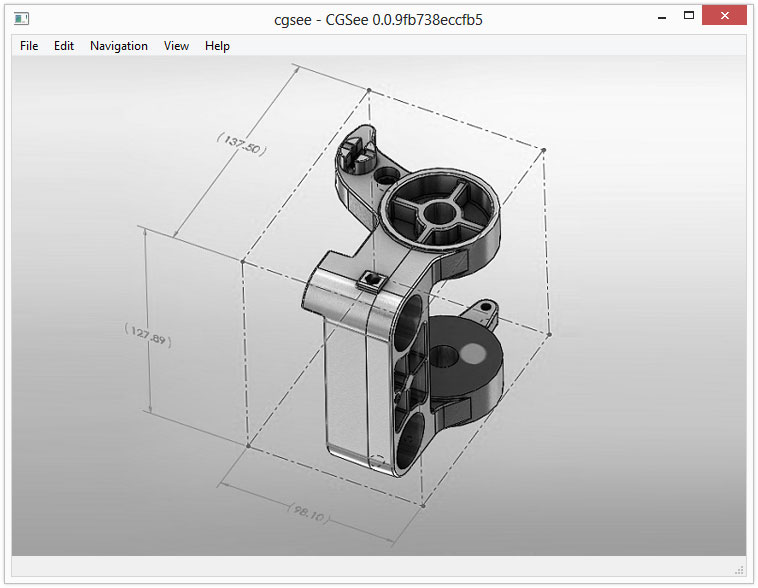
\includegraphics[width=0.3\textwidth]{intro/mock_05}
	~
	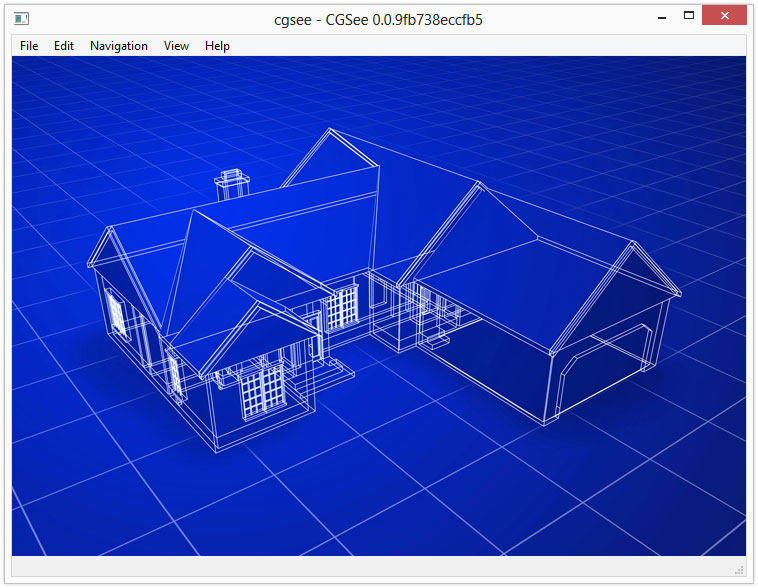
\includegraphics[width=0.3\textwidth]{intro/mock_03}
	~
	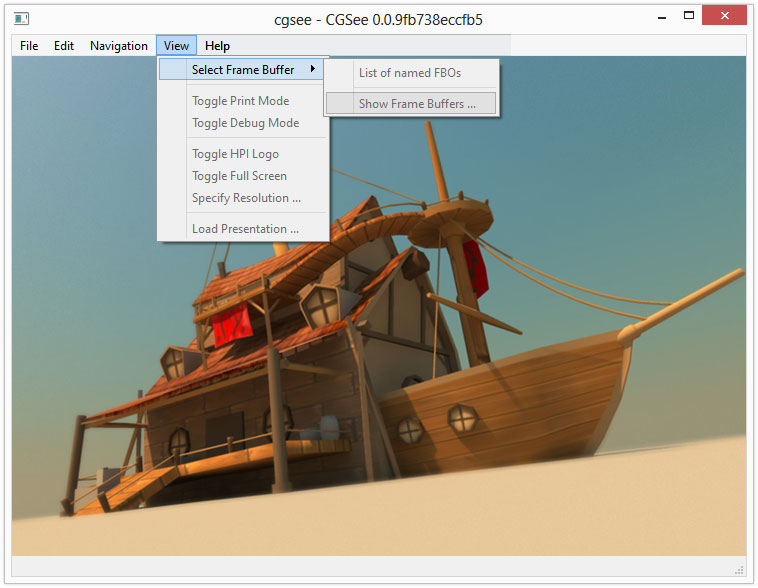
\includegraphics[width=0.3\textwidth]{intro/mock_04}
	
\end{frame}


\begin{frame}{Third Parties, Resources, and Process}

	\begin{columns}

		\begin{column}{0.12\textwidth}

			
\includegraphics[width=\textwidth]{intro/git}
			\medskip

			
\includegraphics[width=\textwidth]{intro/github}
			\smallskip
			
			
\includegraphics[width=\textwidth]{intro/google}
			\smallskip
			
			
\includegraphics[width=\textwidth]{intro/cmake}
			\medskip
			
			
\includegraphics[width=\textwidth]{intro/qt}

		\end{column}
		\begin{column}{0.8\textwidth}

			\textbf{Revisioning} with git\\
			git-scm.com\bigskip
			
			\textbf{Hosted} on github (public)\\
			github.com/cgcostume/cgsee\bigskip

			\textbf{Style Guide} by google\\
			code.google.com/p/google-styleguide\bigskip
			
			\textbf{Project Setup} with CMake\\
			www.cmake.org\bigskip

			\textbf{UI and Rendering} with Qt5 and GLEW\\
			qt-project.org \& glew.sourceforge.net

		\end{column}

	\end{columns}
	
\end{frame}


% -------- -------- -------- -------- -------- -------- -------- --------

\begin{frame}[plain]
	\fullsizegraphic{intro/about}{Participation}
\end{frame}


\begin{frame}{Your Participation}

	Select/Propose at least two tasks. One in C++, the other in rendering with OpenGL.
	\bigskip

	\large
	\textbf{For each task You}
	\begin{enumerate}
	
		\item \textbf{propose} a solution for discussion (during review in hands-on).
		\item \textbf{implement} the (probably refined) solution (2 to 4 weeks).
		\item \textbf{present} your implementation (3 + 2 min).
		\bigskip

		\item pair programming if sufficient number of participants... (group making)
		
	\end{enumerate}

\end{frame}


\begin{frame}{About Grading}
	
	\center
	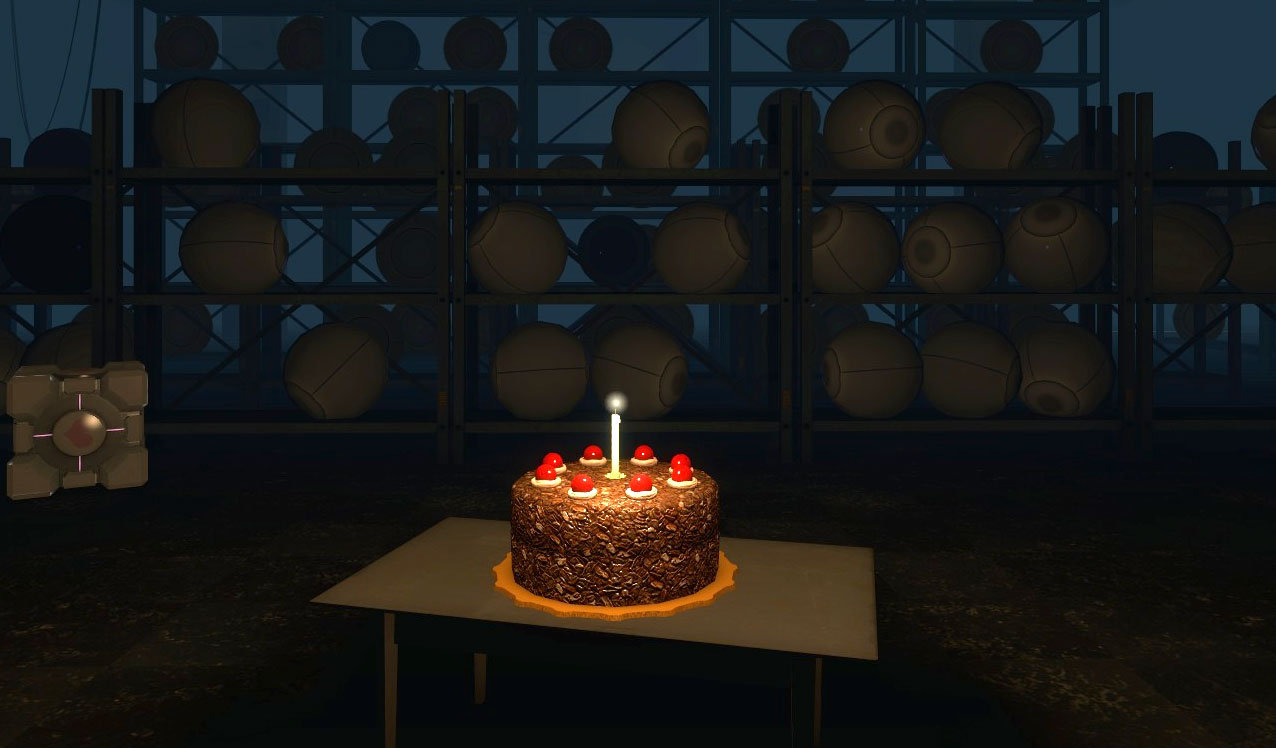
\includegraphics[width=0.6\textwidth]{intro/cake}\medskip

	\LARGE
	$\frac{1}{4}$ task \textbf{presentations} and $\frac{3}{4}$ task \textbf{implementations}	

	\medskip
	\scriptsize
	Actually it's $\frac{2}{8} + \frac{5}{8}$ ... with an added $\frac{1}{8}$ for \textbf{valuable participation}.
	
\end{frame}


% -------- -------- -------- -------- -------- -------- -------- --------

\begin{frame}[plain]
	\fullsizegraphic{intro/ideas}{Get Started}
\end{frame}


\begin{frame}{More Inspiration}

	\center

	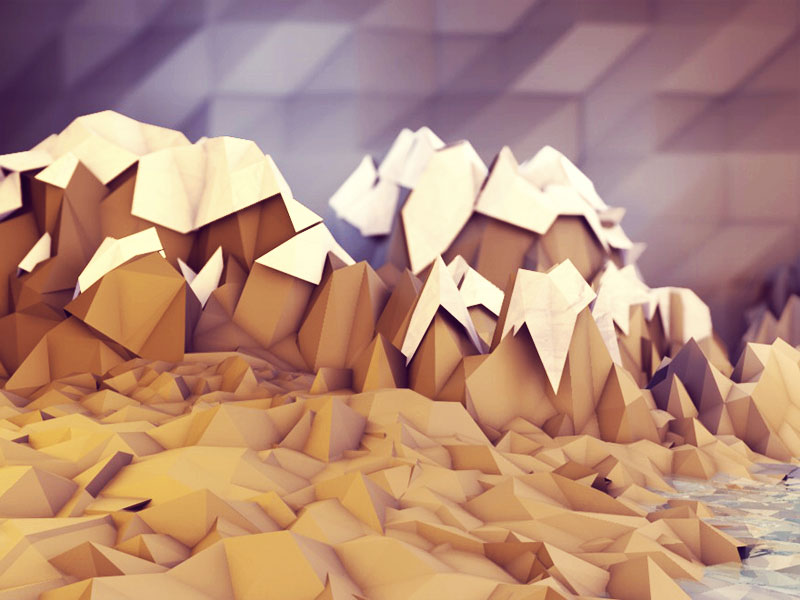
\includegraphics[width=0.3\textwidth]{intro/rendering_00}
	~
	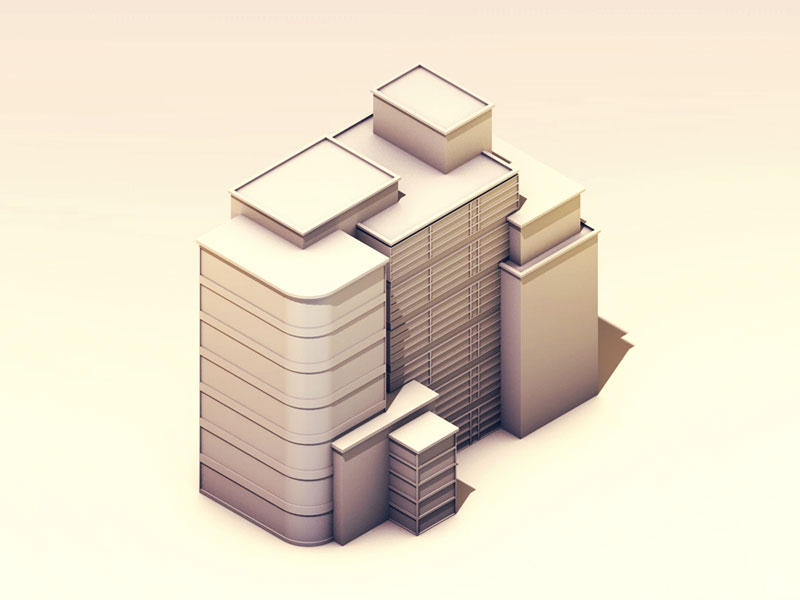
\includegraphics[width=0.3\textwidth]{intro/rendering_01}
	~
	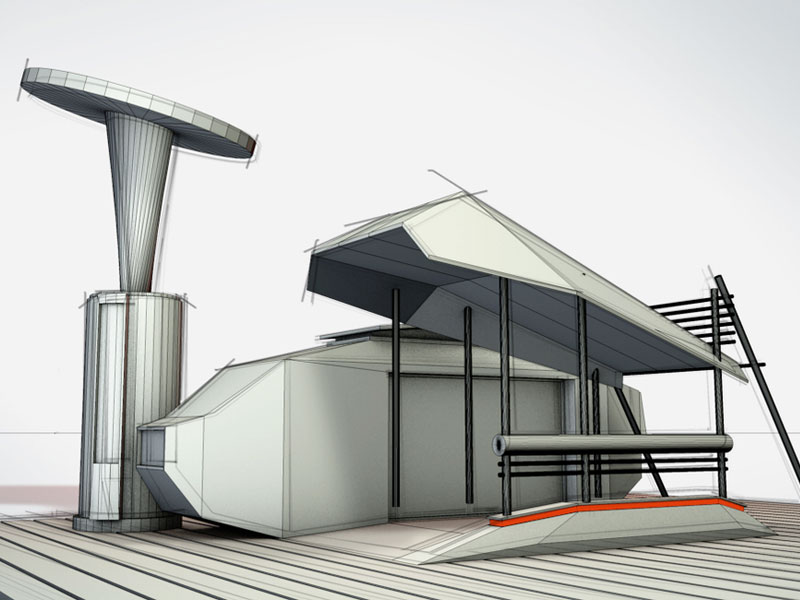
\includegraphics[width=0.3\textwidth]{intro/rendering_02}
		
	\medskip
	
	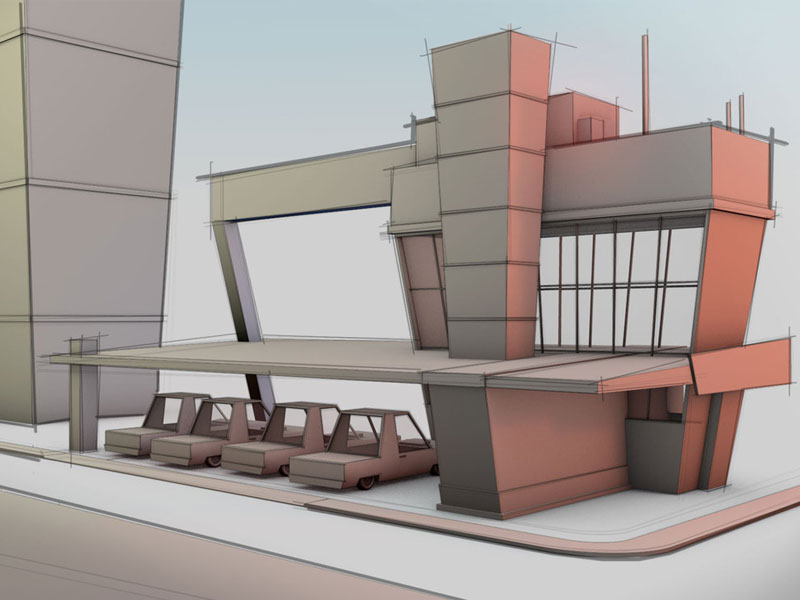
\includegraphics[width=0.3\textwidth]{intro/rendering_05}
	~
	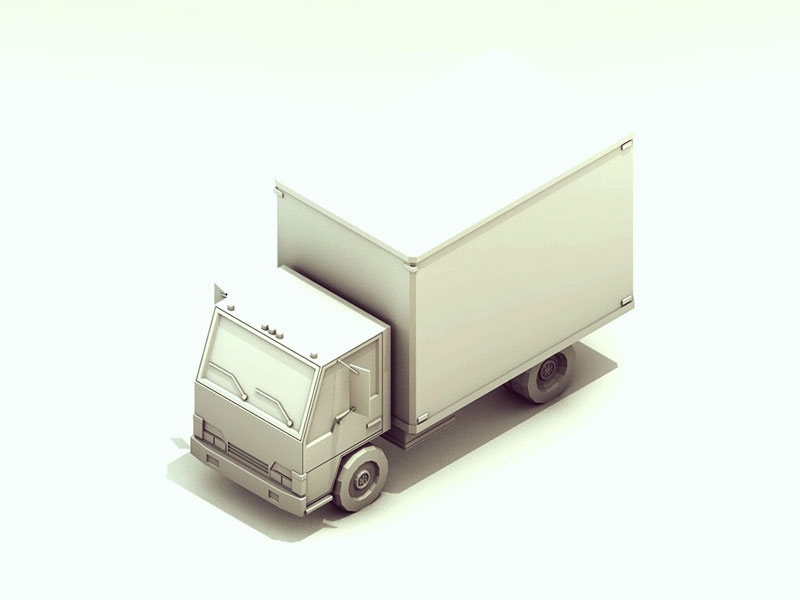
\includegraphics[width=0.3\textwidth]{intro/rendering_04}
	~
	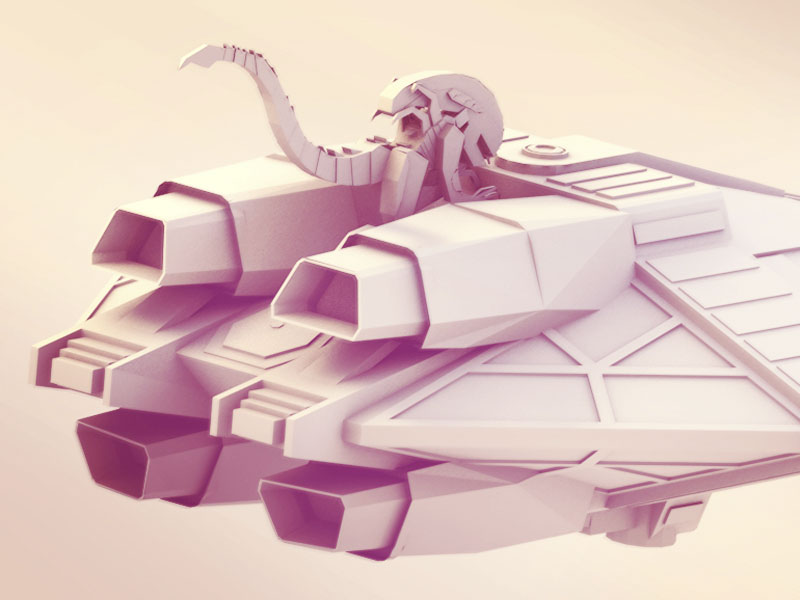
\includegraphics[width=0.3\textwidth]{intro/rendering_03}
	
\end{frame}


\begin{frame}{Issues (Excerpt)}

	\center
	\small

	\begin{columns}[t]
		\begin{column}{0.5\textwidth}

			\pause
			\begin{enumerate}

				\item Data Import and Export
					\begin{itemize}\scriptsize
						\item Image and 3D Formats
						\item Scene Graph and Matrices Provisioning% for Transformation Handling, State Sorting, Intersections, etc.
						\item Materials: Diffuse, Bump, Ambient %Opacity, Specular, Highlight, Ambient, ...)
					\end{itemize}

				\pause
				\item Efficient Scene Rendering
					\begin{itemize}\scriptsize
						\item View Frustum Culling
						\item Scene Graph Traversal / State Sorting
						\item Vertex Cache Optimization
					\end{itemize}

				\pause
				\item Image Based Rendering
					\begin{itemize}\scriptsize
						\item Render To Texture, Antialiasing
						\item Provisioning of Common G-Buffers
						\item Shadows, Grid, Environments, Ground Plane
						\item Lighting, SSAO, Spherical Harmonics
						\item NPR/Stylization: Blue Print, Pencil
					\end{itemize}

			\end{enumerate}

		\end{column}
		\begin{column}{0.5\textwidth}

			\begin{enumerate}
				\setcounter{enumi}{3}
			
				\pause
				\item Interaction and Analysis
					\begin{itemize}\scriptsize
						\item Navigations: Trackball, Flight, Walk %(Trackball, Flight, Terrain, Walk, Drive, Guided, ...)
						\item Bounding Boxes, Dimensions, Cross Sections, Explosion, Coloring
						\item Scene Graph and additional Information Display and Search
						\item Viewport Management and Transitions
						\item View Cube
						\item Measuring and Labeling: Angles, Distances, Ruler, Labels, Volumes
					\end{itemize}
				
				\pause
				\item Manipulation and Creation
					\begin{itemize}\scriptsize
						\item Picking, Hovering, and Highlighting
						\item Selecting, Filtering, Editing (Gizmos) % Scale, Rotate, Translate, Mirror, etc ...
						\item Geometry Fixes: Duplicate Vertices % Vertex Weld, Duplicate Vertices, Triangulation, Triangle Strip Optimizations, ...
						\item Camera Path Editor
					\end{itemize}
			
			\end{enumerate}
	
		\end{column}
	\end{columns}
	\bigskip\bigskip

	\pause
	\large And most importantly, \textbf{YOUR IDEAS!}
	\bigskip

\end{frame}


\begin{frame}{Getting Started on File Formats}

	\center
	\small

	\begin{columns}[t]
		\begin{column}{0.4\textwidth}

			3D Geometry File Formats:\medskip

			\begin{itemize}\scriptsize
				\item 3DS MAX (\textbf{.3ds} and .max)
				\item Autodesk (.fbx)
				\item Auto CAD (.dwg, .dxf)
				\item Alias WavefrontTM (\textbf{.obj})
				\item Blender (.blend)
				\item Cinema 4D (.c4d)
				\item Collada (\textbf{.dae})
				\item DirectX (\textbf{.x})
				\item Lightwave (\textbf{.lwo} and .lws)	
				\item OpenCTM (\textbf{.ctm})
				\item QuakeTM (\textbf{.mdl .md2} and \textbf{.md3})	
				\item SketchUp (\textbf{.skp})
				\item Stanford Polygon PLY (\textbf{.ply})
				\item Extensible 3D (.x3d)
			\end{itemize}

		\end{column}
		\begin{column}{0.3\textwidth}

			2D Image File Formats:\medskip

			\begin{itemize}\scriptsize
				\item Windows Bitmap (\textbf{.bmp})
				\item JPEG (\textbf{.jpg})
				\item Portable RGB (.ppm)
				\item RAW (\textbf{.raw})
				\item TARGA (\textbf{.tga})
				\item PNG (\textbf{.png})
				\item TIFF (\textbf{.tiff})
				\item DXTC (\textbf{.dds})
			\end{itemize}

		\end{column}
	\end{columns}

	\bigskip

\end{frame}


% -------- -------- -------- -------- -------- -------- -------- --------

\begin{frame}[plain]
	\fullsizegraphic{intro/fin}{}
\end{frame}


\begin{frame}{Coming Next}

	\begin{columns}
		\begin{column}{0.5\textwidth}

			\begin{itemize}
				\item CGSee version control with Git.
				\item Building CGSee with CMake on gcc/msvc.
				\item CGSee source code introduction.
				\item Feature planning and issue assignment.
				\item Issue tracking in github.
			\end{itemize}

		\end{column}
		\begin{column}{0.5\textwidth}

			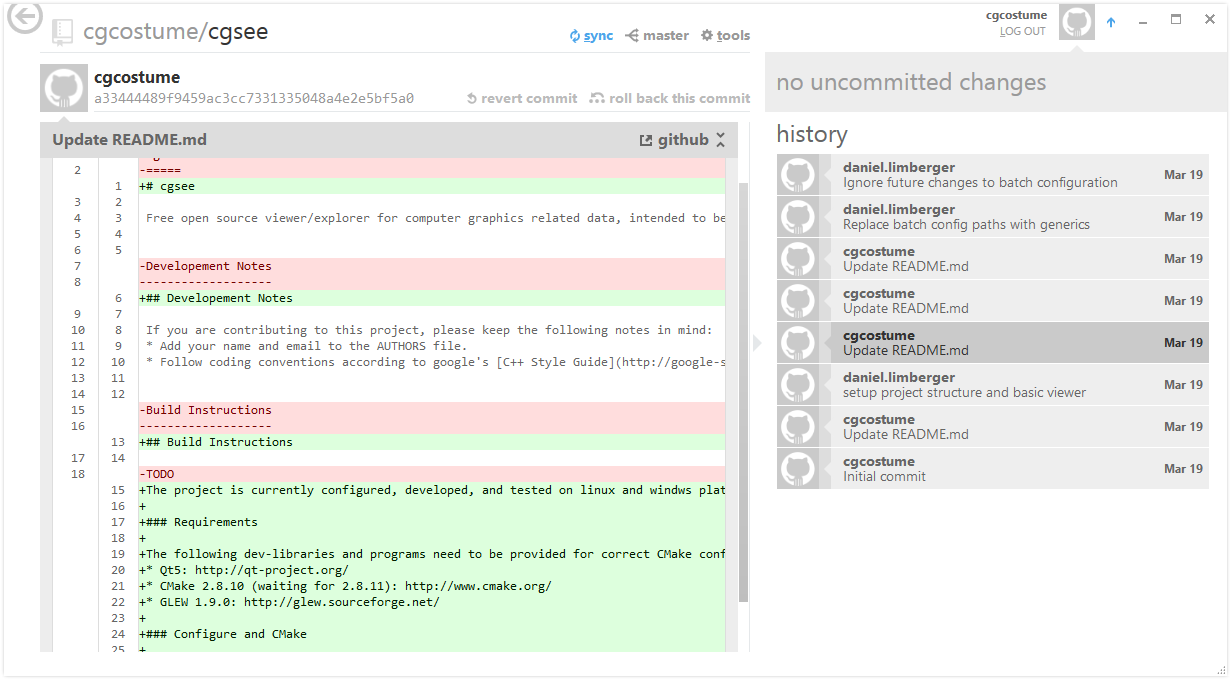
\includegraphics[width=\textwidth]{intro/githubwin}
			
		\end{column}
	\end{columns}

\end{frame}


\begin{frame}{Image Rights}
	
	\begin{itemize}
		\item Teaser 'House' by iStockphoto.com/Martin Fischer
		\item Teaser 'Tepaot' by Hay Kranen / CC-BY
		\item Teaser 'Firefly' by Alex Kung http://www.seansgallery.com/gallery/3dgraphics/serwip24.jpg
		\item OpenGL Guys from OpenGL Quick Reference Card http://www.khronos.org/files/opengl43-quick-reference-card.pdf
		\item Cake from Valve's game Portal
		\item Stanford Bunny in Mock by Jean-Christophe Naour (flickr)
		\item Solidworks Bounding Box from http://cadcamstuff.com/
		\item Boat by Toby Lewin at http://www.tobylewin.com
		\item WTFs/Minute by Tom Holwerda at http://www.osnews.com/comics
		\item Others by Timothy J. Reynolds
	\end{itemize}
	
\end{frame}


\end{document}
